\chapter{Layer 2}
It's the layer responsible of sending packets over the network. As it will be explained in Chapter \ref{layer3} , Layer 3 network disappeared and all local area network are supported by Layer 2. Hence routing isn't needed in the network anymore.\\
When a smartphone connect to a network, uses a Point to Point Layer 2 connection using LTE/4G/5G, and it's connected to Local Network Area (LAN) using WiFi. Layer 2 supports protocols HDLC, PPP(Point to Point Protocol) in Point to Point connections and Ethernet(IEEE 802.3 802.11) in LAN (Local Area Networks).\\
Hence Internet Packet passes only through two types of networks: Point to Point link or Local Area Networks.
\begin{figure}[h]
\centering
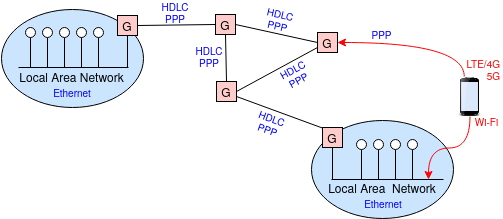
\includegraphics[scale=0.4]{Images/Layer2/layer2}
\caption{\footnotesize{Nowadays L2 connections.}}\label{layer2}
\end{figure}

\section{Ethernet}
In Ethern protocol, there was a coaxiale cable, long about 1.5 km, on which host interconnect (Figure \ref{ethernet}). All the hosts electrically shared a bus. In the past hosts ethernet interfaces were connected through a vampire tap junction but now, they are connect to cable using a T-junction (see Figure \ref{vampire_tap} and Figure \ref{t_junction}). The difference between them is that the first one connects electrically to the cable (connecting it to a cable cut) and the second one is used only in ethernet cables that are physically composed by different cable (segments) and the T-junction is put at intersection of two segments.\\
The protocol supports Carriege Sense Multiple Access Collision Detection (CSMA/CD), used for coordination between hosts, that it's composed by two strategies:
\begin{itemize}
\item{\textbf{Carrier sense}\\
An host can't speak while anyone else is speaking}
\item{\textbf{Collision detection}\\
the protocol resolves conflicts raised during the contention time. Contention time is the time in which people, that respect first rules, can also go in conflict starting talking together at the same moment.}
\end{itemize}
\begin{figure}[h]
\centering
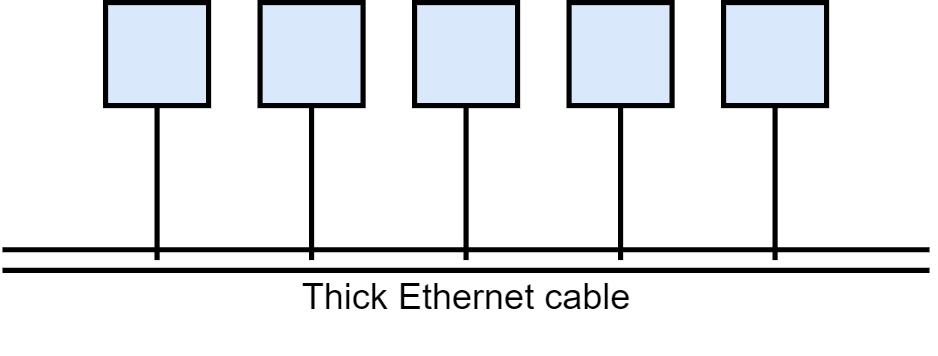
\includegraphics[scale=0.3]{Images/Layer2/ethernet}
\caption{\footnotesize{Ethernet.}}\label{ethernet}
\end{figure}
\begin{figure}[h]
\centering
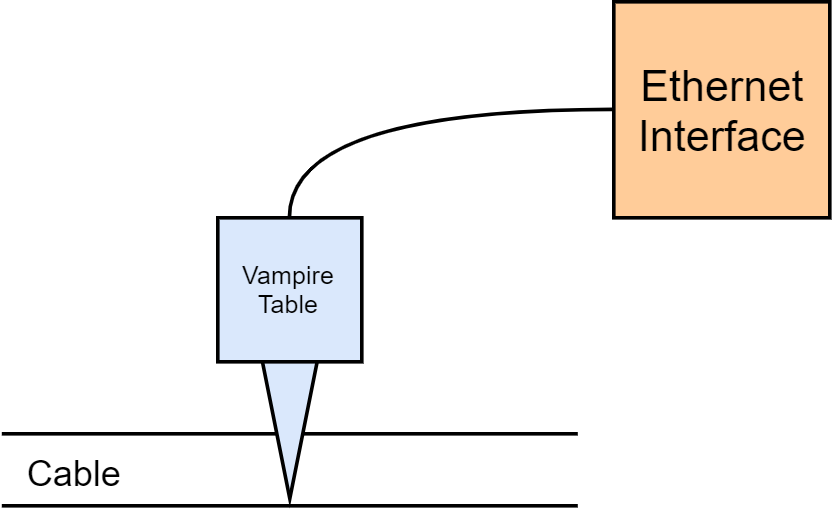
\includegraphics[scale=0.3]{Images/Layer2/vampire_tap}
\caption{\footnotesize{Vampire tap.}}\label{vampire_tap}
\end{figure}
\begin{figure}[h]
\centering
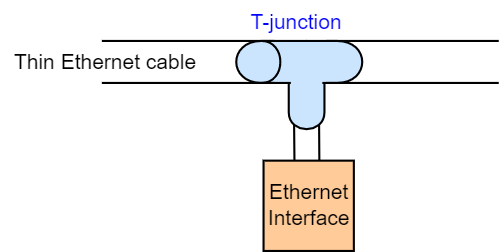
\includegraphics[scale=0.5]{Images/Layer2/t_junction}
\caption{\footnotesize{T-junction.}}\label{t_junction}
\end{figure}
